\section{Optimierung mit einen Evolutionsalgorithmus}
\subsection{Der Evolutionsalgorithmus}
Folgende Quelltexte sind das implementierte Hauptprogramm und die implementierten Funktionen des Evolutionsalgorithmus.

\begin{code}
	\caption{moonLanding}
	\mSourceFile{\srcDir/moonLanding.m}
	\label{fig:moon-landing-m}
\end{code}

\begin{code}
	\caption{initialize.m}
	\mSourceFile{\srcDir/initialize.m}
	\label{fig:initialize-m}
\end{code}

\begin{code}
	\caption{bread.m}
	\mSourceFile{\srcDir/bread.m}
	\label{fig:bread-m}
\end{code}

\begin{code}
	\caption{mutate.m}
	\mSourceFile{\srcDir/mutate.m}
	\label{fig:mutate-m}
\end{code}

\begin{code}
	\caption{evaluate.m}
	\mSourceFile{\srcDir/evaluate.m}
	\label{fig:evaluate-m}
\end{code}

\subsection{Optimierungen des Evolutionsalgorithmus}
\subsubsection{Implementierung}
Die Aufteilung der Aufgaben des Algorithmus wurden wie ind er Übung bereits gemacht übernommen. Ein Lösungskandidat wird mit $fac_{punish}$ bestraft wenn $minH > 0$, da hier der Boden nicht erreicht wurde und daher dieser Lösungskandidat nicht zu gut bewertet werden darf. Wenn $1/5$ der Lösungskandidaten bessere Lösungen gefunden hat als die letzte Generation, dann $\delta = \delta - \delta_{step}$ ansonsten $\delta = \delta + \delta_{step}$. Damit wird die Schrittweite zusätzlich erhöht oder verkleinert. 
\newline
\newline
Am ende des Programms werden die besten und der Durchschnitt der Qualitäten je Generation in einem Chart angezeigt, um so den Verlauf der Suche der Lösungskandidaten zu veranschaulichen.

\subsubsection{Was muss optimiert werden ?}
Es müssen Werte für die Parameter des Algorithmus wie z.B $\mu$, $\lambda$, $\delta$ und $\delta_{step}$ gefunden werden, mit denen die Wahrscheinlichkeit hoch ist gute Lösungskandidaten zu bekommen. Prinzipiell muss der Algorithmus von der konkreten Problemstellung nichts wissen, jedoch spielt es eine Rolle wie der Lösungsraum vom Algorithmus durchsucht wird und ob mit diesem Verhalten gute Lösungskandidaten zu ermitteln sind.
\newline
\newline
Aufgrund der möglichen langen Laufzeit sollte auch Parallelisierung in Betracht gezogen werden, was in dieser Übung nicht angewandt wurde.

\subsubsection{Was ist eine geeignete Fitnessfunktion ?}
Eine gute Fitnessfunktion ist eine Funktion, die in der Lage ist, die Lösungskandidaten je nachdem ob sie gute oder schlechte sind entsprechend zu bewerten. Die Bewertung wird im Algorithmus dazu verwendet um zu ermitteln wie hoch der Anteil an guten Lösungskandidaten war und aus welchen Lösungskandidaten eine neue Generation erzeugt wird.

\subsubsection{Welche Parameter können modifiziert werden ?}
Folgende Auflistung zeigt die Parameter, die modifiziert werden können:
\begin{itemize}
	\item $\mu$ ist die Anzahl der Elter aus denen in einer Generation Mutanten erzeugt werden.
	\item $\lambda$ ist die Anzahl der zu erzeugenden Mutanten pro Elter pro Generation
	\item $\delta$ ist die maximale Schrittweite, um die sich ein Parameter in einem Parametervektor pro Mutation ändern darf.
	\item $\delta_{step}$ ist das Delta, mit dem die Schrittweite pro Generation zusätzlich vergrößert wird, je nachdem ob eine neue beste Lösung gefunden wurde oder nicht.
	\item $maxUnsuccessCount$ ist die maximale Anzahl von nicht neu gefunden besten Lösungskandidaten pro Generation.
	\item $maxGenerationCount$ ist die maximale Anzahl von Generationen, die der Algorithmus durchläuft.
	\item $initialVektor$ ist der initiale Parametervektor, mit dem der Algorithmus gestartet wird.	
\end{itemize}

\subsubsection{Warum ein Evolutionsalgorithmus ?}
Im Gegensatz zu einem \emph{Particle Swarm} Algorithmus muss ein Evolutionsalgorithmus den Lösungsraum nicht kennen und der Lösungsraum muss kein Koordinatensystem sein. Ebenso ist ein \emph{Particle Swarm} Algorithmus nicht anwendbar auf Optimierungsprobleme, was aber eine Mondlandung ist. Im Gegensatz zu einem \emph{Tabu} Algorithmus benötigt ein Evolutionsalgorithmus kein Gedächtnis. Ein Evolutionsalgorithmus ist auch an sich schon dafür geeignet reelwertige Vektoren zu optimieren und kann auf Optimierungsprobleme angewendet werden. 
\newline
\newline
Die Annäherung an gute Lösungskandidaten erfolgt schrittweise pro Generation in dem die besten Lösungskandidaten pro Generation herangezogen werden, um die nächste Generation zu erzeugen. Die Schrittweite um die sich die Werte eines Parametervektors pro Mutation ändern können, wird beeinflusst ob man einen guten Lösungskandidaten nahe ist oder nicht (\emph{pro Generation eine neuer bester Lösungskandidat}).

\subsection{Testfälle mit verschiedenen Konfigurationen}
Die folgenden Test stellen verschiedene Konfigurationen gegenüber wie $\lambda$, $\delta$, $\delta_{step}$ und die Anzahl der maximalen Generationen und der maximalen fehlerhaften Durchläufe. Im Chart wird die beste Konfiguration pro Generation mit ihrer Qualität angezeigt. Gibt es keine Veränderung zwischen zwei Generationen, so hat es auch keinen neuen besten Lösungskandidaten in dieser Generation gegeben. Für die genau Konfiguration eines Tests siehe bitte die Abbildung.
\newpage

\subsubsection{Test 1}
\begin{figure}[h]
	\centering
	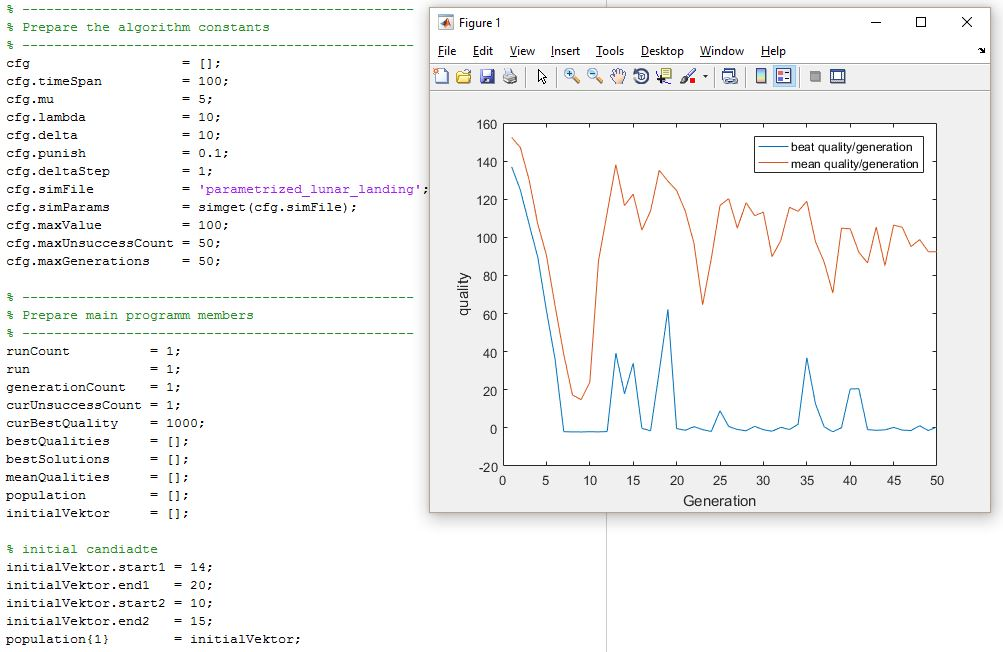
\includegraphics[scale=0.45]{\imageDir/simulink-luna-landing-paramterized-test-1.JPG}
	\caption{$\mu=5, \lambda=10, \delta=10, \delta_{step}=1, punish=0.1, mGen=50, mUnsuc=50 $}
	\label{fig:simulink-luna-landing-paramterized-test-1}
\end{figure}

\subsubsection{Test 2}
\begin{figure}[h]
	\centering
	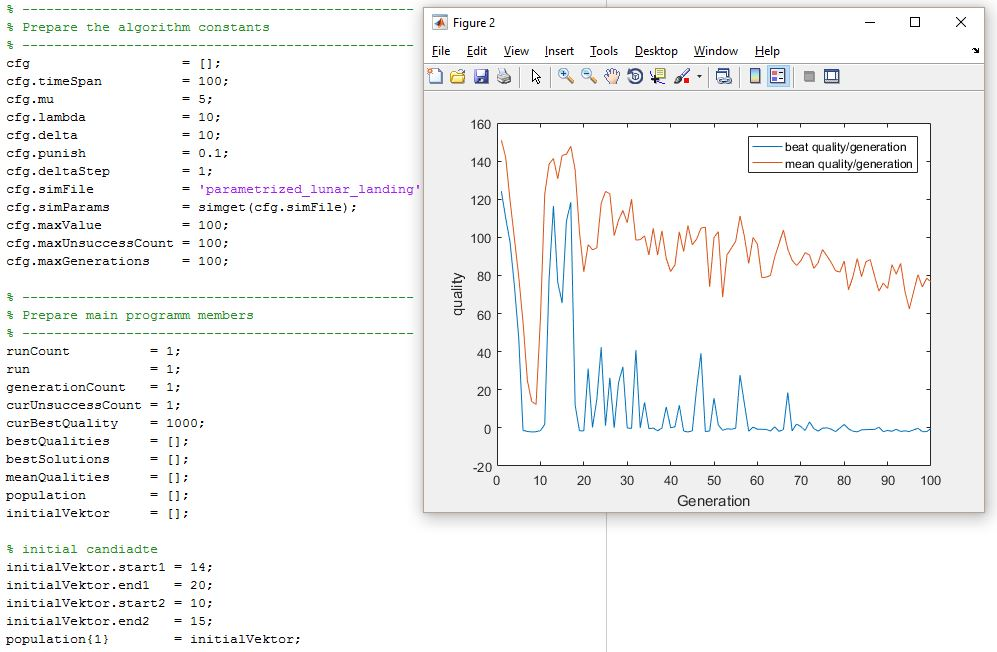
\includegraphics[scale=0.45]{\imageDir/simulink-luna-landing-paramterized-test-2.JPG}
	\caption{$\mu=5, \lambda=10, \delta=10, \delta_{step}=1, punish=0.1, mGen=100, mUnsuc=100 $}
	\label{fig:simulink-luna-landing-paramterized-test-2}
\end{figure}
\ \newpage

\subsubsection{Test 3}
\begin{figure}[h]
	\centering
	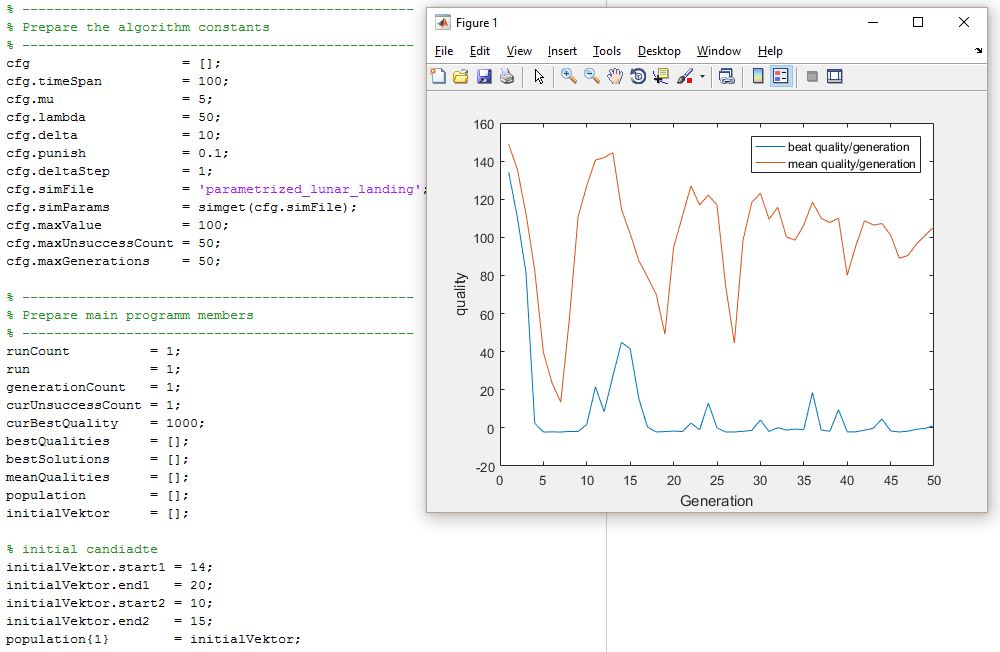
\includegraphics[scale=0.45]{\imageDir/simulink-luna-landing-paramterized-test-3.JPG}
	\caption{$\mu=5, \lambda=50, \delta=10, \delta_{step}=1, punish=0.1, mGen=50, mUnsuc=50 $}
	\label{fig:simulink-luna-landing-paramterized-test-3}
\end{figure}

\subsubsection{Test 4}
\begin{figure}[h]
	\centering
	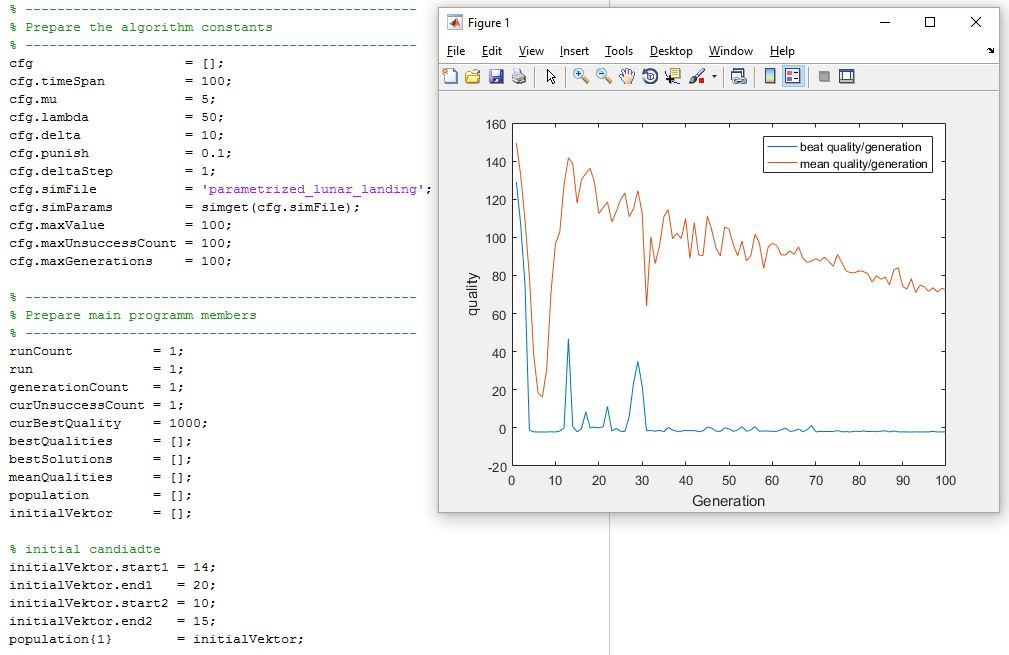
\includegraphics[scale=0.45]{\imageDir/simulink-luna-landing-paramterized-test-4.JPG}
	\caption{$\mu=5, \lambda=50, \delta=10, \delta_{step}=1, punish=0.1, mGen=200, mUnsuc=100 $}
	\label{fig:simulink-luna-landing-paramterized-test-4}
\end{figure}
\ \newpage

\subsubsection{Test 5}
\begin{figure}[h]
	\centering
	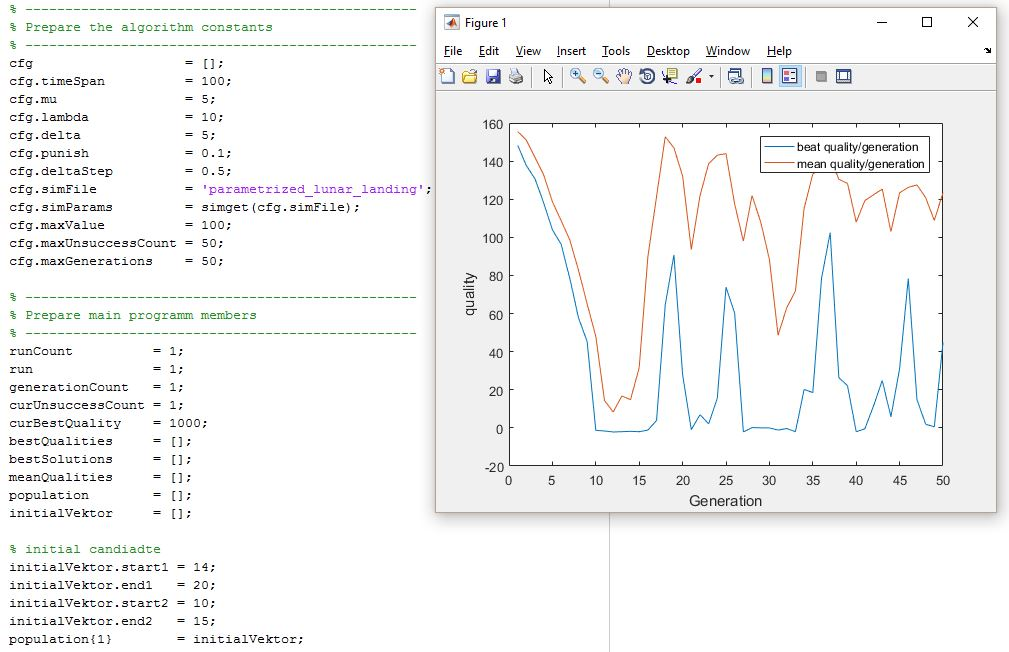
\includegraphics[scale=0.45]{\imageDir/simulink-luna-landing-paramterized-test-6.JPG}
	\caption{$\mu=5, \lambda=10, \delta=5, \delta_{step}=0.5, punish=0.1, mGen=50, mUnsuc=50 $}
	\label{fig:simulink-luna-landing-paramterized-test-5}
\end{figure}

\subsubsection{Test 6}
\begin{figure}[h]
	\centering
	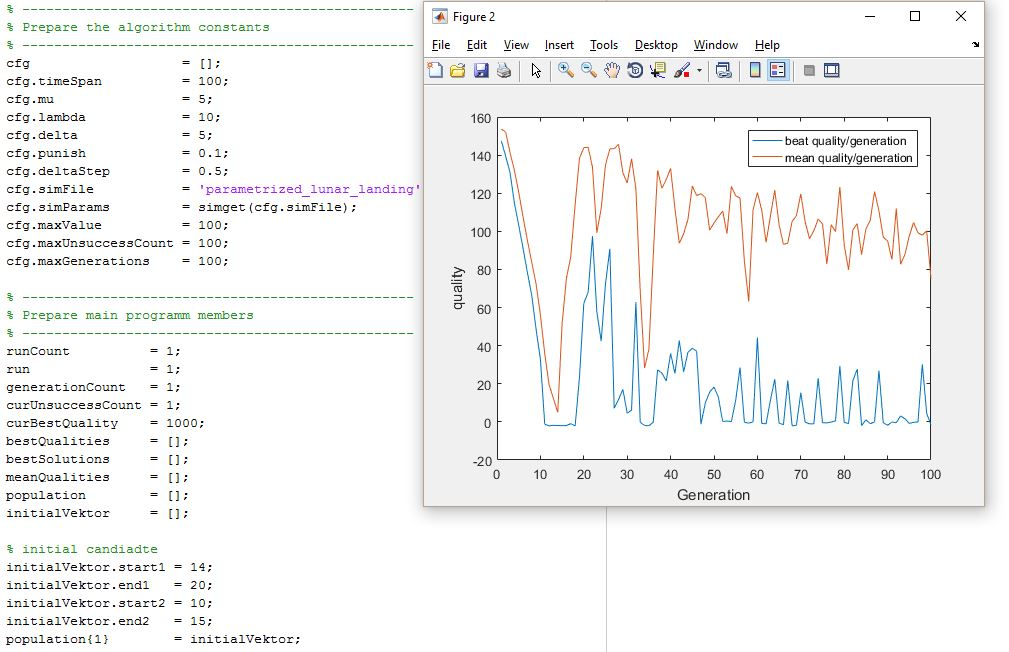
\includegraphics[scale=0.45]{\imageDir/simulink-luna-landing-paramterized-test-5.JPG}
	\caption{$\mu=5, \lambda=10, \delta=5, \delta_{step}=0.5, punish=0.1, mGen=100, mUnsuc=100 $}
	\label{fig:simulink-luna-landing-paramterized-test-6}
\end{figure}
\ \newpage

\subsubsection{Test 7}
\begin{figure}[h]
	\centering
	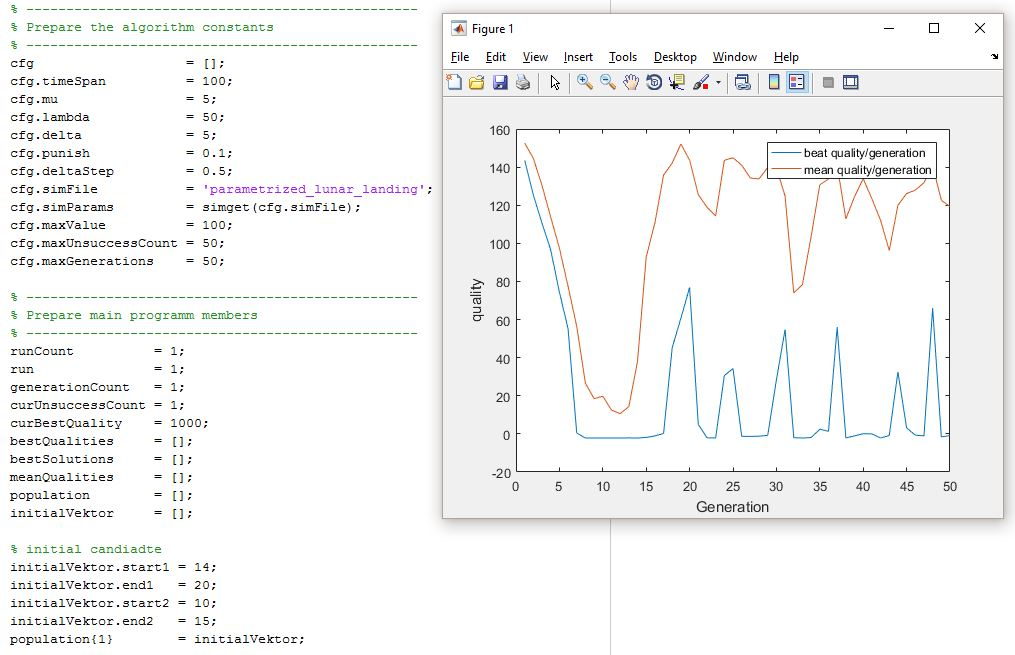
\includegraphics[scale=0.45]{\imageDir/simulink-luna-landing-paramterized-test-7.JPG}
	\caption{$\mu=5, \lambda=50, \delta=5, \delta_{step}=0.5, punish=0.1, mGen=50, mUnsuc=50 $}
	\label{fig:simulink-luna-landing-paramterized-test-7}
\end{figure}

\subsubsection{Test 8}
\begin{figure}[h]
	\centering
	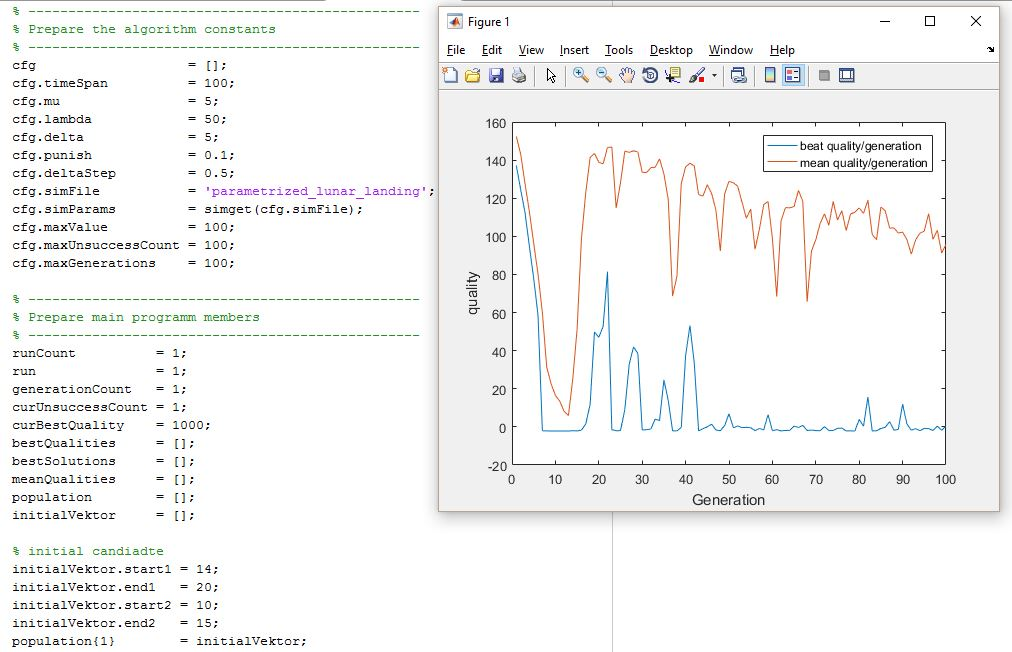
\includegraphics[scale=0.45]{\imageDir/simulink-luna-landing-paramterized-test-8.JPG}
	\caption{$\mu=5, \lambda=50, \delta=5, \delta_{step}=0.5, punish=0.1, mGen=100, mUnsuc=100 $}
	\label{fig:simulink-luna-landing-paramterized-test-8}
\end{figure}
\ \newline
Die Tests zeigen dass mit einem zu kleinen $\mu$ zu viele Lösungskandidaten nicht gefunden werden können. Ebenso muss die Anzahl der Generationen groß genug sein, damit genügend Lösungen durchprobiert werden können.  